\documentclass[a4paper,12pt]{article}
\usepackage{amsmath}
\usepackage{amssymb}
\usepackage[polish]{babel}
\usepackage{polski}
\usepackage[utf8]{inputenc}
\usepackage{indentfirst}
\usepackage{geometry}
\usepackage{array}
\usepackage[pdftex]{color,graphicx}
\usepackage{subfigure}
\usepackage{afterpage}
\usepackage{setspace}
\usepackage{color}
\usepackage{wrapfig}
\usepackage{listings}
\usepackage{datetime}

\renewcommand{\onehalfspacing}{\setstretch{1.6}}

\geometry{tmargin=2.5cm,bmargin=2.5cm,lmargin=2.5cm,rmargin=2.5cm}
\setlength{\parindent}{1cm}
\setlength{\parskip}{0mm}

\newenvironment{lista}{
\begin{itemize}
  \setlength{\itemsep}{1pt}
  \setlength{\parskip}{0pt}
  \setlength{\parsep}{0pt}
}{\end{itemize}}

\newcommand{\linia}{\rule{\linewidth}{0.4mm}}

\definecolor{lbcolor}{rgb}{0.95,0.95,0.95}
\lstset{
    backgroundcolor=\color{lbcolor},
    tabsize=4,
  language=C++,
  captionpos=b,
  tabsize=3,
  frame=lines,
  numbers=left,
  numberstyle=\tiny,
  numbersep=5pt,
  breaklines=true,
  showstringspaces=false,
  basicstyle=\footnotesize,
  identifierstyle=\color{magenta},
  keywordstyle=\color[rgb]{0,0,1},
  commentstyle=\color{blue},
  stringstyle=\color{red}
  }

\begin{document}

\noindent
\begin{tabular}{|c|p{11cm}|c|} \hline 
Grupa 4 & Barbara Nowak, Piotr Tomaszewski & \ddmmyyyydate\formatdate{26}{10}{2016} \tabularnewline
\hline 
\end{tabular}


\section*{Zadanie 1 - Macierze OMP}

Celem naszego zadania było zaimplementowanie programu, którego zadaniem jest obliczenie iloczyn dwóch macierzy kwadratowych wypełnionych liczbami losowymi wg wzorów podanych w specyfikacji zadania. Do zrównoleglenia obliczeń wykorzystaliśmy bibliotekę OpenMP.



Program uruchamiany jest z dwoma argumentami: \quotedblbase ilWatkow\textquotedblright - to liczba wątków a \quotedblbase rozmiarMac \textquotedblright- to rozmiar macierzy. Pierwszym i bardzo ważnym etapem w naszym programie jest sprawdzenie poprawności wprowadzanych danych przed przystąpieniem do wykonywania obliczeń.

\begin{lstlisting}
void liczenieMacierzy(double **AAA, double **BBB, double **CCC, int rozmiarMac){
	int i,j,k;

	#pragma omp parallel for default(none) shared(AAA, BBB, CCC) firstprivate(rozmiarMac) private(i, j, k)
	for (i = 0; i < rozmiarMac; i++) {
		for (j = 0; j < rozmiarMac; j++) {			
			for (k = 0; k < rozmiarMac; k++) {
				CCC[i][j] += AAA[i][k] * BBB[k][j];	//obliczanie iloczynu - algorytm naiwny
			}
		}
	}
}
\end{lstlisting}

Zadaniem powyższej funkcji jest pomnożenie elementów macierzy A i B a następnie zapisanie wyniku do macierzy C. Do przyspieszenia obliczeń użyto dyrektywy OpenMP w celu zrównoleglenia pętli. Dyrektywa ta składa się z parametrów:
\textbf{parallel} - wskazanie kompilatorowi obszaru kodu, który będzie zrównoleglany; 
  \textbf{omp} - słowo kluczowe odnoszące się do OpenMP; 
  \textbf{for} - zrównoleglana będzie pętla for; 
  \textbf{default(none)} - ustawienie domyślnego zasięgu zmiennych wewnątrz równolegle przetwarzanego obszaru, gdzie parametr "none" narzuca deklarowanie każdej zmiennej;  
  \textbf{shared} - określenie wspólnych zmiennych (zmienne, do których kazdy wątek ma dostęp); 
  \textbf{private} - określenie zmiennych prywatnych (zmienne, do których tylko jeden wątek ma dostęp);
  \textbf{firstprivate} - określenie zmiennych prywatnych już zainicjowanych.



\begin{lstlisting}
#pragma omp parallel for default(shared)
\end{lstlisting}
Powyższa dyrektywa różni się, od zastosowanej w kodzie programu, tym, że zmienne są współdzielone. Polega to na tym, że w procesie zrównoleglania zmienne będą musiały być ciągle synchronizowane pomiędzy wątkami. Oczywiście uzyskamy przyspieszenie w obliczeniach ale nie tak efektywne. Dyrektywa zastosowana w programie określa jasno, które zmienne ma traktować jako prywatne a które są współdzielone, przez co program nie musi tracić czas na synchronizację.

\begin{lstlisting}
omp_set_num_threads(ilWatkow); 			

startTime = omp_get_wtime(); 			
liczenieMacierzy(AAA, BBB, CCC, rozmiarMac);	
stop = omp_get_wtime(); 		
\end{lstlisting}

Powyższy fragment kodu jest odpowiedzialny za ustawienie liczby wątków dla zrównoleglnych obszarów, ustawienie momentu uruchomienia pomiaru czasu wykonywanego zadania, uruchomienie funkcji mnożącej dwie macierze oraz ustalenie zakończenia pomiaru czasu.

\begin{wrapfigure}{r}{0.5\textwidth}
	\vspace{-40pt}
	\begin{center}
		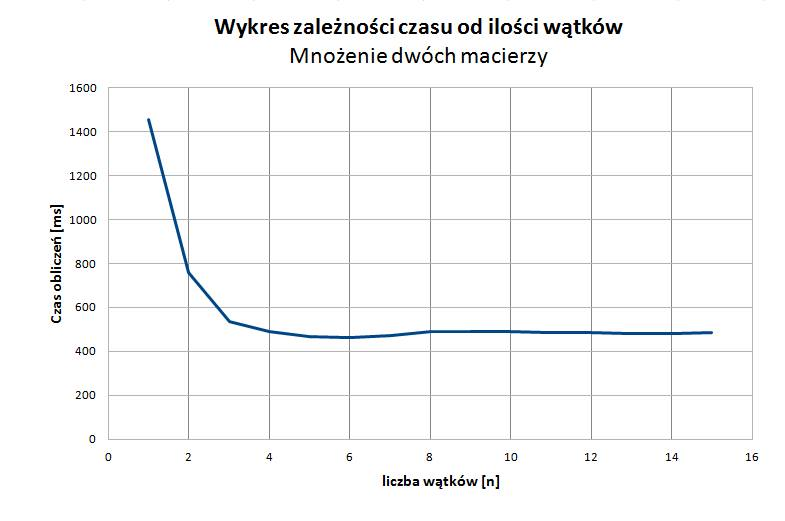
\includegraphics[width=0.5\textwidth]{img1.jpg}
	\end{center}
	\vspace{-20pt}
	\caption{Wykres zależności czasu od liczby wątków}
	\vspace{35pt}
\end{wrapfigure}

Do celów ćwiczeniowych, nasze macierze przyjeliśmy o rozmiarz \textit{500x500}. Wykres zależności czasu od liczby wątków (Rysunek 1) dla mnożenia macierzy A i B, ukazuje, że wraz ze wzrostem liczby wątków czas obliczeń znacznie spada. Przy czterech wątkach czas łagodnie i płynnie opada aż do osiągnięcia stabilnego poziomu. 

Proces zrównoleglenia przy pomocy biblioteki OpenMP również bardzo dobrze obrazuje poniższy wykres przyspieszenia (Rysunek 2). Widzimy tutaj, że program przyspiesza aż do osiągnięcia ośmiu wątków a następnie zrównolegla się. Serwer uruchomieniowy jest wyposarzony w 4-rdzeniowy procesor z technologią Hyper-Threading dlatego pozwalająca mu pracować na 8 wątkach.

\begin{wrapfigure}{r}{0.5\textwidth}
	\vspace{-40pt}
	\begin{center}
		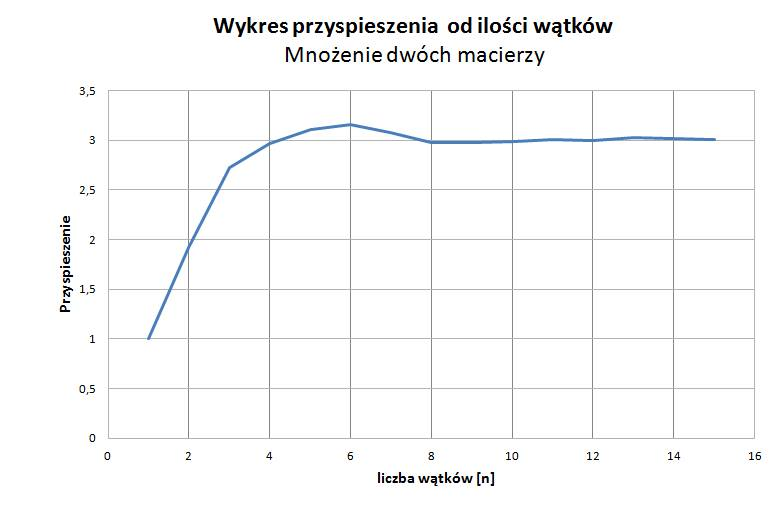
\includegraphics[width=0.5\textwidth]{img2.jpg}
	\end{center}
	\vspace{-20pt}
	\caption{Wykres przyspieszenia}
	\vspace{35pt}
\end{wrapfigure}


\textbf{Podsumowanie:} OpenMP to rozszerzenie dla języków C/C++ pozwalające mieć wpływ na programowanie wielowątkowe. Każdy z wątków może posiadać własny tymczasowy widok na wspólny obszar pamięci. Zmienne zawarte w bloku parallel można podzielić na private - zmienne do których tylko jeden wątek ma dostęp i shared - dostęp wielu wątków do zmiennych. Używanie większej ilości wątków niż jest to sprzętowo możliwe to nie najlepsze rozwiązanie. Można pomyśleć, że przy nieskończonej ilości wątków czas będzie dążył do zera - to nie jest prawda. Po przekroczeniu możliwości procesora, czas wykonywania programu wzrośnie. Przy wykonywaniu obliczeń występowały zawahania czasowe - spowodowane było tym że kilka osób jednocześnie wykonywało pracę. Rozwiązaniem tego problemu było ponowne uruchomienie obliczeń.


\end{document}
